%!TEX root = Nanomat.tex
\ctitletwo{Cushing: Produksjon av nanopartikler med kjemiske metoder}
\addcontentsline{toc}{section}{CUSHING - PRODUKSJON AV NANOPARTIKLER MED KJEMISKE METODER}
\cstitletwo{Solvotermisk prosessering}
\paragraph{Autoklave} En autoklave er rett og slett en forseglet boks. En typisk autoklave består av en container av polytetrafluoroetylen (teflon) omsluttet av et tykt stålskall, med et tykt skrulokk av stål som er boltet fast med stålskruer. Her er en figur som beskriver alt du egentlig trenger å vite om en autoklave:
\begin{figure}[H]
	\centering
	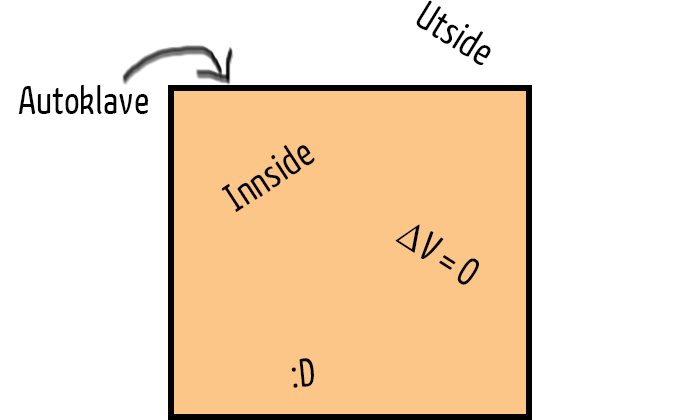
\includegraphics[width=0.95\linewidth]{autoklave.png}
	\label{fig:autoklave}
\end{figure}
Til våre formål er en autoklave den beste fysiske tilnærmingen til et lukket system:  volum og masse holdes konstant, mens temperatur kan kontrolleres utenfra. Autoklaver gjør det mulig å oppnå høyt trykk ved å øke temperaturen. Dette høye trykket gjør det mulig å utføre reaksjoner ved lavere temperaturer enn man ellers ville trengt.

\paragraph{Solvotermisk prosessering} er kjemiske prosesser som utføres i en lukket beholder (for eksempel en autoklave), slik at økt temperatur også medfører økt trykk.\footnote{Siden $pV=nRT$ og sånn. Altså, $pV$ er overhodet ikke lik $nRT$ i de fleste syntesene som beskrives her, siden vi ser på crazy blandinger av superkritiske fluider, surfaktanter, fast stoff og alt mulig rart, egentlig alt annet enn ideelle gasser. Uansett: det stemmer fortsatt at hvis $\Delta p > 0$ så er også $\Delta T > 0$.} Dette er betingelser som gir de oppløste stoffene \emph{økt løselighet og økt reaktivitet}.

Noen ganger økes trykk og temperatur såpass at man får et superkritisk løsemiddel, men ofte trenger man ikke å føre løsemiddelet forbi det kritiske punktet for å oppnå det man ønsker.

Slik bruk av en autoklave har flere fordeler:
\begin{itemize}
	\item Løselighet øker med trykk, så det høye trykket i en autoklave gjør at man oppnår en løselighet som man ellers ville trengt en langt høyere temperatur for å oppnå. Dermed kan man syntetisere materialer som ville blitt ustabile ved høye temperaturer.
	\item Reaksjonsproduktene er ofte krystalline, og trenger ikke den samme etterbehandlingen som man trenger ved bruk av kopresipitering eller sol-gel-metoder (som vi kommer til i de neste delkapitlene).
	\item En lukket beholder er et miljø der man presist kan kontrollere betingelser som pH og konsentrasjon av reaktanter.
\end{itemize}

For å utdype det siste punktet: her er en oversikt over hvordan forskjellige betingelser påvirker det endelige produktet. Det er dessverre få forklaringer på \emph{hvorfor} det er slik, men det finner man altså heller ikke mye av i Cushing.
\begin{itemize}
	\item Høy temperatur gir en bred fordeling av partikkelstørrelser. Lav temperatur gir en smal fordeling av partikkelstørrelser.
	\item Mineraliserende stoffer fører til redusert gjennomsnittlig partikkelstørrelse. De brukes også fordi de hjelper med å stabilisere forløperne og mellomproduktene i reaksjonen. Samtidig fører de også til agglomerering. Typiske mineraliserende stoffer er hydroksider, karbonater og halider.
	\item Aminer fungerer som ``capping agents'', som hindrer partikler fra å vokse forbi en viss maksimumstørrelse. Slike ``capping agents'' kan også forhindre agglomerering.
	\item Partikler vokser i størrelse over tid,\footnote{Hvis det var noen tvil.} så man kan kontrollere størrelsen ved å kontrollere tiden.
	\item Høy konsentrasjon av forløper gir høy faserenhet. Lav konsentrasjon fører til blandede faser.
	\item Krystallstrukturen til partiklene påvirkes av pH.
\end{itemize}

\paragraph{Hydrotermisk prosessering} er et spesialtilfelle av solvotermisk syntese der løsemiddelet er vann.

\paragraph{Mikrobølgeassistert solvotermisk prosessering} Man kan bruke mikrobølger til å forårsake veldig rask oppvarming av reaksjonsblandingen -- særlig hvis den inneholder vann. Dette gjør at partikler presipiterer raskt og nesten samtidig, som igjen gjør at partiklene blir veldig små, og har en smal størrelsesfordeling. Dette er en metode som brukes for å lage oksider og zeolitter (som vi skal snakke om i neste kapittel).

% Eks hydrot. syntese av kvarts: NaOH for å solubilisere silica ved lave T

% Autoklaver - gir kontrllert
% pH (kontrollere krystallstruktur)
% T (kontrollere dispersitet)
% t eller addisjon av surfaktaner/ioner (kontrollere størrelse)
% c (høyere konsentrasjon gir høyere phase purity)

% Continuous flow hydrothermal reactor
% X: mixing point: Ce-precursor, Zr-precursor, H20 near critical point
% PH: pre-heater, C: cooler, F filter

% Microwave-assisted solvothermal processing: what?

\paragraph{Presipitering og kopresipitering} Presipitering (eller utfelling) er dannelsen av fast stoff i løsning under en kjemisk reaksjon, typisk fordi reaksjonsproduktet har lavere løselighet i løsemiddelet enn reaktantene har. Kopresipitering er år flere forskjellige kjemiske specier presipiterer samtidig, og så danner mer komplekse systemer. Et eksempel på kopresipitering er når to forskjellige metaller presipiterer i samme løsning samtidig.

\paragraph{Egenskaper til utfellingsreaksjoner} Den vanligste måten å forårsake utfelling på, er kjemiske reaksjoner der produktet har lav løselighet i løsningen, slik at løsningen raskt blir overmettet. I slike reaksjoner er nukleering det viktigste trinnet. Sekundære effekter som Oswald ripening og agglomegering kan ha stor effekt på det endelige produktet. Reaksjonsbetingelser (for eksempel hvor raskt man legger til reaktanter, eller hvor raskt man rører i løsningen) kan naturligvis også påvirke det endelige resultatet.

\paragraph{Dispersjon} En dispersjon er et system der en kjemisk forbindelse er dispergert (det vil si at den finnes i form av finfordelte partikler) i en fase med en annen kjemisk sammensetning. Eksempler på dispersjoner er
\begin{itemize}
	\item Suspensjon, en dispersjon av partikler av fast stoff i væske.
	\item Sol, en dispersjon av kolloidale partikler av fast stoff i væske. Altså en suspensjon der partiklene er kolloider.
	\item Emulsjon, en dispersjon av væske (i veldig små dråper) i en annen væske.
\end{itemize}

\paragraph{Reduksjon av metall i løsning} En vanlig metode for å lage metall-nanopartikler er å \emph{redusere metalliske salter}. For å redusere et metallisk salt kreves det at endringen i fri energi er negativ. Dersom vi har standardbetingelser vil det si at cellepotensialet fra elektrokjemien, altså
\begin{equation}
	E^o_{\text{celle}} = E^o_{\text{reduksjon}} + E^o_{\text{oksidasjon}}
\end{equation}
skal være \emph{positivt}. Som regel har vi \emph{ikke} standardbetingelser, og må erstatte halvcellepotensialene i ligningen over med
\begin{equation}
	E = E^o - \frac{RT}{nF}\ln Q.
\end{equation}
Men dette er vi jo kjent med fra kjemi.

En metode for å sørge for at endringen i fri energi er negativ, er å bruke reduksjonsmidler. Noen vanlige reduksjonsmidler \emph{i vandig løsning} er:
\begin{itemize}
	\item Hydrogengass
	\item Solvaterte borohydridsalter, altså \ce{ABH4}, der \ce{A} er et alkalimetall
	\item Hydrasinhydrat \ce{N2H4.H2O} eller hydrasindihydro\-klorid \ce{N2H4.2HCl}\hfill
	\item Aminer
	\item Karboksylsyrer
	\item Alkoholer
\end{itemize}
Vann er ikke alltid egnet som løsemiddel. Hvis metallet er langt nede i spenningsrekka, altså edelt, kan man ikke bruke vann som løsemiddel.  Et reduksjonsmiddel som er kraftig nok til å redusere kationer fra et edelt metall, vil også være sterkt nok til å redusere vann i reaksjonen \ce{2H2O+2e- <-> H2+2OH-}, som har en $E^o=\SI{-0.8277}{\volt}$. Da må vi bruke ikke-vandige løsninger. Noen vanlige reduksjonsmidler \emph{i ikke-vandig løsning} er:
\begin{itemize}
 	\item \ce{NaBH4} og \ce{H2}, som før
 	\item DMF (N,N-dimetylformamid)
 	\item Alkoholer (særlig hvis vi har sterkt oksiderende kationer)
 	\item Alkalider, altså komplekser med alkalimetall-anioner som \ce{Na-}
 	\item Elektrider, altså komplekser med solvaterte elektroner (\ce{e- (aq)}, liksom). Solvaterte elektroner er det sterkeste reduksjonsmidlet som det er teoretisk mulig å lage.
 \end{itemize}
En annen grunn til å bruke ikke-vandige løsninger er at det ikke er alle produkter som er stabile i vandig løsning (eller mer generelt polare løsninger). For eksempel er kolloidale gullpartikler ikke stabile i polare løsninger. Men det kan fortsatt være gunstig å starte med en vandig løsning. Her er et eksempel på en prosess der man bruker både vandig og ikke-vandig løsning, for å lage kolloidale partikler av gull:
\begin{enumerate}
	\item Lag en vandig løsning med \ce{AuCl4-}
	\item Overfør \ce{AuCl4-} til en organisk fase ved å blande den vandige løsningen kraftig sammen med en løsning av tetraoktylammoniumbromid i toluen.
	\item Legg til dodekantiol i den organiske fasen. Dette er surfaktantene som blir sittende utenpå de kolloidale partiklene.
	\item Legg til en vandig løsning av \ce{NaBH4}. Dette blir redusjonsmiddelet. Rør kraftig.
	\item Det dannes kolloidalt gull med størrelse mellom 1 og 3 nm. La dette felles ut av løsningen.
	\item Isoler produktet som et tørt pulver. Ved å tilføre et uploart løsemiddel (eller et svakt polart et, som toluen) kan du få tilbake en stabil løsning av kolloidale gullpartikler.
\end{enumerate}

\paragraph{Andre metoder for å redusere metall} Det finnes noen andre metoder:
\begin{itemize}
	\item \emph{Elektrokjemisk reduksjon}, der metallet reduseres på en katode gjennom elektrolyse. Her trenger man et stabiliserende stoff for å unngå at metallet bare deponerer som en film på katoden.
	\item \emph{Strålingsassistert reduksjon}, der man bruker ioniserende lys til å spalte stoffer og lage radikaler, solvaterte elektroner og lignende. Disse kan så redusere metallet.
\end{itemize}

\paragraph{Utfelling av oksider fra vandig løsning} For å lage nanopartikler av krystalline oksider (hydroksider, karbonater, bikarbonater, oksalater, o.l.) kan vi få metallkationer til å kopresipitere, og så kalsinere dem. Det finnes to kategorier av reaksjoner som produserer oksider:
\begin{itemize}
	\item De som produserer et oksid direkte
	\item De som produserer en egnet forløper til et oksid. Forløperen må deretter prosesseres for å lage oksidet.
\end{itemize}
Det som er vanskelig ved utfelling av oksider er ikke å få til reaksjonen, men å få monodisperse partikler. Ved utfelling av oksider trenger man gjerne en stabilisator bundet til overflaten for å unngå aggregering. Med denne metoden kan man lage materialer som har funky støkiometriske formler (typ \ce{La_{$1-x$}Sr_$x$NbO4}), og kan fungere som
\begin{itemize}
	\item Protonledende elektrolytter
	\item Oksygenion-ledende elektrolytter
	\item Blandede ledere
	\item Anoder
	\item Katalysatorer
\end{itemize}

\paragraph{Utfelling av oksider fra ikke-vandig løsning} I vandig løsning bruker man ofte pH for å trigge utfelling. Hvis man trenger metaller som presipiterer ved veldig forskjellige pH må man bruke en ikke-vandig løsning. Ikke-vandige løsninger vil også forhindre prematur presipitering av hydroksider, som er vanlig i høyvalente kationer som \ce{Ti4+} og \ce{Zr4+}. Vanlige forløpere med denne metoden er tertiære metall-alkoksider, altså \ce{M(OR)4}. Dette er en bra metode for å lage bariumtitanat \ce{BaTiO3}. 

\cstitletwo{Sol-gel-prosessering}
Sol-gel er, kort forklart, \emph{hydrolyse og konsensering av metall-alkoksider}. Et metallalkoksid er noe som er på formen \ce{M(RO)_{$x$}}, altså en konjugerende base til et alkohol. Vi lager primært \emph{metalloksider} med denne metoden.

\paragraph{Aerogel!} Før vi går inn på metoden må det sies at det er sånn her man lager aerogel. Aerogel er et superluftig materiale som består av ultraporæst silisiumoksid. Det har et stort indre overflateareal og ekstremt lav varmeledningsevne. Det brukes derfor til varmeisolering, til tynnfilmer på selvrensende vinduer og til å samle støv fra kometer.

\paragraph{Metode} Sol-gel-syntese skjer i seks trinn:
\begin{enumerate}
	\item Dannelse av \emph{sol}, en løsning av metall-alkoksider eller metallkomplekser.
	\item Dannelse av \emph{gel}, et nettverk med oksid- eller alkohol-broer. Dette skjer ved polykondensering eller polyforestring.
	\item \emph{Aldring} (synerese), som skjer når polykondensasjonen har nådd punktet der gel-en er en solid masse. Gel-nettverket trekker seg sammen og gjør veggene sterkere, og noe av løsemiddelet fjernes.
	\item \emph{Tørking}: vann og andre flyktige væsker fjernes
	\item \emph{Dehydrering}: \ce{M-OH}-grupper på overflaten fjernes. Dette hindrer gel-en fra å rehydrere. Skjer ved ca. \SI{800}{\celsius}.
	\item Det siste trinnet skjer kun hvis man skal lage en xerogel for å lagge tette keramer eller glass. nemlig \emph{densification} der temperaturen er høyere enn \SI{800}{\celsius}. Porene i gel-nettverket kollapser, organiske specier fjernes.
\end{enumerate}
De første to trinnene bestemmer komposisjonen til det endelige materialet. 

\paragraph{Kjemiske reaksjoner i sol-gel-syntese} Det er to viktige reaksjoner som skjer i sol-gel-syntese:\footnote{Denne forklaringen av sol-gel-kjemi er ikke særlig bra. Beklager.}
I \emph{hydrolyse}trinnet erstatter man en \ce{OR}-gruppe med en \ce{OH}-gruppe ved å legge til vann i løsningen. Hydrolyse kan skje enten i sur eller i basisk løsning - det vil være enten \ce{H+}-ioner eller \ce{OH-}-ioner som katalyserer reaksjonen. Hydrolyse skjer saktere i sur løsning enn i basisk løsning. Antall \ce{OR}-grupper som hydrolyseres på alkoksidet kalles \emph{hydrolyseringsgraden}, og denne avhenger av forholdet mellom metall-forløper og vann. Mye vann fører til høyere hydrolyseringsrad. For eksempel, for TEOS (tetraetylortosilikat):
\begin{equation}
	\ce{ Si(OR)4 + nH2O -> Si(OR){4-n}(OH)n+nROH }
\end{equation}
Under \emph{kondensering}strinnet dannes det en polymer gjennom polykondensasjon. Kondensasjonsreaksjonen kan enten være \emph{alkoksalering} eller \emph{oksalering}. Veldig forenklet kan man si at alkoksalering er når det lages en binding mellom \ce{OR}-gruppen til ett metall-alkoksid og \ce{OH}-gruppen til et annet metall-alkoksid samtidig som man spalter av en \ce{ROH} --- mens oksalering er når det lages en binding  \ce{OH}-gruppene til to metall-alkoksider samtidig som man spalter av en \ce{H2O}. Oksalering er mye raskere fordi \ce{OH}-gruppen er en bedre utgående gruppe enn \ce{OR}.

Hydrolyseringsgraden $n$ bestemmer hva slags produkt man får. Når $n=1$ får man dimerer, hvis $n=2$ får man 1-dimensjonale kjeder eller 2-dimensjonale ringer, og hvis $n=4$ får man 3-dimensjonale nettverk og fraktaler. 

\paragraph{Effekten til pH} Årsaken til at pH har noe å si for strukturen det endelige produktet, er at \emph{hydrolysen skjer raskere i basisk løsning}. Når hydrolysen skjer raskt, vil det tidlig dannes mange hydrolyserte grupper som kan kondensere. Dette gjør at det tidlig dannes forgreinede molekyler og klynger som lager tette nettverk på liten skala. Etter hvert som kondensasjonen fortsetter, vil strukturen vokse ved at forskjellige klynger går sammen, så man får et nettverk av klynger.

I sur løsning skjer hydrolysen tregere. Dette gjør at de kondenserte molekylene er mer lineære tidlig i prosessen. Det er først senere i prosessen at de møter hverandre og danner et sammenvevd nettverk. 

\paragraph{Endelige produkter} Det finnes tre typer endelige gels, som klassifiseres etter styrken av det inorganiske nettverket:
\begin{itemize}
	\item I en \emph{xerogel} er nettverket svakt, og det kollapser under tørking. Dette skjer når løsemiddelet har høy overflatespenning, slik at det ``drar'' på gel-nettverket (i form av kapillærkrefter) når det tørker.
	\item I en \emph{ambigel} har man en mellomting mellom en xerogel og en ambigel. Dette får man når løsemiddelet har lav overflatespenning, slik at løsemiddelet ikke drar så mye på nettverket under tørking.
	\item I en \emph{aerogel} er nettverket sterkt, og beholder nettverksstrukturen under tørking. Dette kan man få ved å bruke et superkritisk fluid som løsemiddel, da et superkritisk fluid ikke har overflatespenning.
\end{itemize}
Gel-en kan være det endelige produktet, eller det kan være en forløper som kalsineres eller sintres for å lage produkter som tette nanokrystalline keramer eller tette filmer.

De vanligste produktene i sol-gel-syntese er oksider, men man kan også lage ting som karbider, nitrider og sulfider. I så fall må man unngå hydrolysen da dette per definisjon gir oksider. Da bør man bruke et aprotisk, inert løsemiddel i stedet for vann.

%Produksjon av komposittmaterialer:  % Eksempler: kvanteprikker i silicatynnfilm
%\begin{enumerate}
%	\item 
%	\item 
%	\item 
%\end{enumerate}

\paragraph{Pechini-metoden} er en alternativ sol-gel-prosess for metaller som ikke lar seg hydrolysere så lett, for eksempel alkalimetaller, jordalkalimetaller og overgangsmetaller.\footnote{Så... egentlig alt unntatt aluminium, gallium, indium, selen, titan, bly og vismut.} Med Pechini-metoden bruker man organiske ting som sitronsyre, som lager komplekser med disse metallene. Man legger også til et polyaklohol som glykol. Gel-en dannes i dette tilfellet gjennom en polyforestring der sitronsyre og glykol inngår, mens metallet bare slenger seg på sitronsyra. Etter at man har tørket gel-en kan man varme det opp for å bryte ned det organiske stoffet og få et agglomerat av oksidpartikler.

Problemet med denne metoden er at det er vanskelig å kontrollere størrelse, form og morfologi, og at man stort sett får sfærise partikler. Derfor brukes denne metoden først og fremst for å lage fine partikler som deretter kan sintres for å danne tette keramer. Sintring kommer vi til i kapittel 21.

Denne metoden brukes for å lage \ce{BaTiO3}.